%-*- mode: LaTeX; TeX-engine: xetex -*-
\documentclass{beamer}
\usetheme{epiukbbonn}

\usepackage[orientation=landscape, size=a3, scale=1]{beamerposter}

\usepackage{polyglossia}
\setmainlanguage{english}

\usepackage{fontspec}
\setsansfont{Arial}

\renewcommand{\emph}{\textbf}

%\beamertemplategridbackground[1cm]
%\setbeamertemplate{itemize item}{}

\setbeamertemplate{bibliography item}{}

\usepackage[
backend=biber,
style=authoryear,
maxnames=2,
maxbibnames=4,
url=false,
doi=false,
isbn=false,
firstinits=true
]{biblatex}


 \renewbibmacro*{date+extrayear}{%
     \iffieldundef{year}
       {}
       {\printtext[parens]{\printfield{labelyear}\printfield{extrayear}}}}%

% \DeclareNameAlias{byeditor}{sortname}
% % have last names first in all cases
% \DeclareNameFormat{sortname}{%
%    \ifuseprefix
%      {\usebibmacro{name:last-first}{#1}{#4}{#5}{#8}}
%      {\usebibmacro{name:last-first}{#1}{#4}{#6}{#8}}%
%    \usebibmacro{name:andothers}}
 \renewbibmacro*{in:}{}
% % Do not print numbers and eids
 \renewbibmacro*{volume+number+eid}{%
   \printfield{volume}}
 % Do not print notes
 \renewbibmacro*{note+pages}{%
   \setunit{\addcolon}%
   \printfield{pages}%
   \newunit}
% % Do not decorate the title
 \DeclareFieldFormat[article,book,inbook,incollection]{title}{\textit{#1}}
 \DeclareFieldFormat{journaltitle}{#1}
 \DeclareFieldFormat[article]{pages}{#1}
 \DeclareListFormat{language}{}
 \DeclareFieldFormat{booktitle}{#1}
\addbibresource{poster.bib}

\usecaptiontemplate{
\small
\structure{\insertcaptionname~\insertcaptionnumber:}
\insertcaption
} 


\linespread{1.02}
\newenvironment{wideitemize}{\itemize\addtolength{\itemsep}{.2em}\addtolength{\labelsep}{.1ex}}{\enditemize}

\title{Sample Title}
\author{A. Author\textsuperscript{1}, V. A. Coenen\textsuperscript{2}, C. E. Elger\textsuperscript{1}, M. Soehle\textsuperscript{3}, F. Mormann\textsuperscript{1}}
\institute{\textsuperscript{1}Dept. of Epileptology, \textsuperscript{2}Stereotaxy and MR based OR Techniques, Dept. of Neurosurgery, \textsuperscript{3}Dept. of Anaesthesiology and Intensive Care Medicine, University of Bonn, Germany\\ Presentation THE NUMBER - Contact: THE EMAIL}

\begin{document}
\begin{frame}[t]
\begin{columns}[T]
\begin{column}{.32\linewidth}
\begin{block}{Overview}
\begin{columns}[T]
\begin{column}{.35\linewidth}
\emph{Background}\vspace{\itemsep}
\begin{wideitemize}
\item Item 1
\item Item 2
\item 
\item 
\item 
\end{wideitemize}
\end{column}
\begin{column}{.52\linewidth}
\emph{Main research question}
\begin{wideitemize}
\item What is your question?
\end{wideitemize}
More text!


\emph{Secondary research questions}

\emph{Approach}

\end{column}
\end{columns}
\end{block}

\begin{block}{Methods}
\begin{columns}[T]
\begin{column}{.33\linewidth}
\emph{Patients}
\begin{wideitemize}
\item We obtained micro-electrode recordings from 11~neurosurgical patients undergoing epilepsy monitoring
\item Patients were implanted with intracerebral micro-electrodes (as in \cite{mormann_latency_2008})
\item
\item 
\end{wideitemize}

\end{column}
\begin{column}{.55\linewidth}
\emph{More Info}
\begin{wideitemize}
\item Anaesthesia was induced solely by a target-controlled infusion of propofol (as in \cite{schnider_influence_1998})
\item 
\end{wideitemize}
\end{column}
\end{columns}

\end{block}

\begin{block}{Methods: Micro-electrode Recordings}
\begin{columns}[T]
\begin{column}{.55\linewidth}
\emph{Micro-electrode recordings}
\begin{wideitemize}
\item Each clinical electrode was equipped with 8~micro-electrodes protruding from its tip
\item Electrodes were located bilaterally in the hippocampus, amygdala, entorhinal cortex, and parahippocampal cortex
\item Unit activity was extracted and spike-sorted with a custom program based on wave\_clus \parencite{quian_quiroga_unsupervised_2004}
\item Please cite Combinato if you used it
%\item Sampling rate: 32~kHz, effective recording bandwidth: 0.1~Hz to 9~kHz
\end{wideitemize}
\end{column}
\begin{column}{.35\linewidth}
\begin{figure}
\label{fig:electrodes}
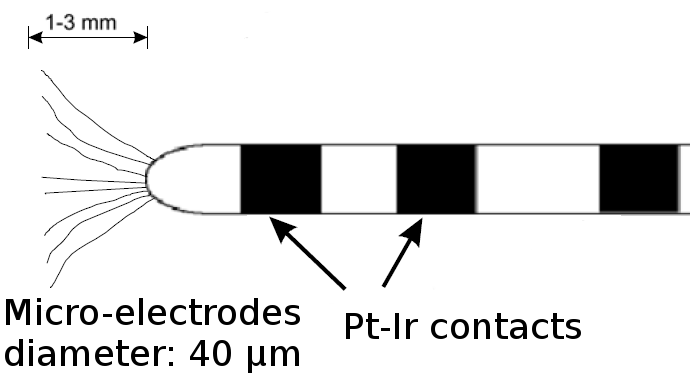
\includegraphics[width=.9\linewidth]{electrodes.png}
\caption{Schematic drawing of electrode with protruding micro-wires}
\end{figure}
\end{column}
\end{columns}
\end{block}



\end{column}
\begin{column}{.32\linewidth}

\begin{block}{Resultsl}
\begin{columns}[T]
\begin{column}{.95\linewidth}
\emph{Dataset}
\begin{wideitemize}
\item Analysis is based on a total of 
\item Unit distribution: 
\end{wideitemize}

\emph{Overall effect of}
\begin{wideitemize}
\item 
\end{wideitemize}
\begin{figure}
\label{fig:proptimecourse}
\begin{center}
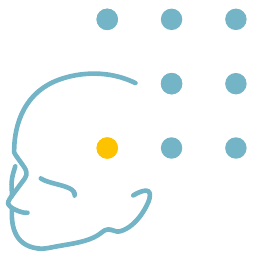
\includegraphics[width=.2\linewidth]{logo-epi.png}
\end{center}
\caption{A bit of a caption}
\end{figure}
\end{column}
\end{columns}
\end{block}
\begin{block}{Results: More}
\begin{columns}
\begin{column}{.95\linewidth}
More text

\begin{figure}
\label{fig:severalunits}
\begin{center}
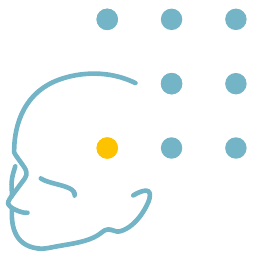
\includegraphics[width=.2\linewidth]{logo-epi.png}
\end{center}
\caption{Yet more text}
\end{figure}
\end{column}
\end{columns}
\end{block}


\end{column}

\begin{column}{.32\linewidth}
\begin{block}{Results}
\begin{columns}[T]
\begin{column}{.95\linewidth}
\begin{wideitemize}
\item We defined \emph{loss of consciousness} as
\item 
\item 
\item 

\end{wideitemize}

\end{column}
\end{columns}
\vspace{2em}


\begin{columns}[T]
\begin{column}{.45\linewidth}
\emph{Firing rate at loss of consciousness}
\begin{wideitemize}
\item For each patient, we calculated
\item Variability between patients was high
\item The relative firing rate is not significantly different from 1 (t-test, P > .27, N = 9)
\item A possible interpretation is that continued neuronal firing at baseline rate
\end{wideitemize}
\end{column}
\begin{column}{.4\linewidth}

\end{column}

\end{columns}
\end{block}
\begin{block}{Further Aims}
\begin{wideitemize}
\item
\item 
\end{wideitemize}
\end{block}
\begin{block}{References}
\begin{columns}[T]
\begin{column}{.8\linewidth}
\setbeamercolor{normal text}{fg=black}
\setbeamercolor{structure}{fg=black}
\appto\bibfont{\small}\printbibliography
\vspace{2.68ex}
\end{column}
\end{columns}
\end{block}

\end{column}
\end{columns}

\end{frame}
\end{document}